%===================================== CHAP 3 =================================

\chapter{Simulation Results}

\section{Simulator}
Often used in control theory, computer simulation is a powerful tool utilized for a variety of purposes. It can be used during development of control schemes during tuning and implementation, and to verify results. As an example for this thesis, running simulations of a control implementation to verify how the control input performs in terms of magnitude and rate is recommended to ensure physically viable control signals and to protect the actuator system from excessive strain.  In order to achieve reliable results from simulations, the simulator should be implemented in such a way that it represents the real world conditions as close as possible, including noise, disturbances and other environmental influences. In the matter of this thesis, the goal of the simulator implementation is to approximate the conditions in the lab. A block diagram of the simulator is shown in Fig. \ref{fig:Simulator} 

\begin{figure}[!h]
\centering
\includegraphics[width=0.8\textwidth]{fig/Simulator.jpg}
\caption{Simulator block diagram}
\label{fig:Simulator}
\end{figure}

To implement the simulator, a mathematical model of the system is needed. In this thesis the system model from Chapter 2.1 is implemented as the function 
\begin{align}
    \Dot{\boldsymbol{\nu}} = \boldsymbol{M}^{-1}(\boldsymbol{\tau} - \boldsymbol{C*\nu} - \boldsymbol{D*\nu}),
\end{align}
where the model matrices $\boldsymbol{M,C}$ and $\boldsymbol{D}$ are given by the uncertainty relation between real and considered model in Eq. \ref{eq:uncert}. The variable $\Dot{\boldsymbol{\nu}}$ is integrated to get velocity measurement $\boldsymbol{\nu}$, and rotated about z then integrated to get position $\boldsymbol{\eta}$. In addition to model uncertainty, the uncertainty associated with the actuators is parameterized as $\boldsymbol{\tau}^*$ = $\rho \boldsymbol{\tau}$.

In addition to uncertainties begin present, it is a known fact that the measurement signals in the lab are susceptible to noise. In order to replicate the same noise in the simulator, an analysis of the noisy data is needed. A sample of position and velocity data from an earlier experiment in the lab is used for the analysis. By examining the Power Spectral Density (PSD) of the position signal shown in Fig. \ref{fig:PSD}, one can see that the noise is most significant in the frequency range close to 20Hz. As the aim is to replicate the conditions in the lab, the same PSD profile should be introduced to the simulator measurements. By bandpass-filtering band limited white noise and adding it to band limited white noise of higher power, the noise profile is approximately recreated, as seen in Fig. \ref{fig:PSD}. The PSD is found using the Fast-Fourier-Transform (FFT). 

\begin{figure}[!h]
\centering
\includegraphics[width=0.8\textwidth]{fig/PSD.jpg}
\caption{Reconstructed noise profile for position measurement}
\label{fig:PSD}
\end{figure}

The power of the white noise used is displayed in Table \ref{table:}. Note that the power of the noise in the y-measurement is set higher than in the x-measurement. This is due to the setup of the positioning system in the lab.


\section{Results}

\subsection{$\mathcal{L}_1$ Adaptive Control}

\subsection{Immersion and Invariance Adaptive Control}
\begin{figure}[!h]
\centering
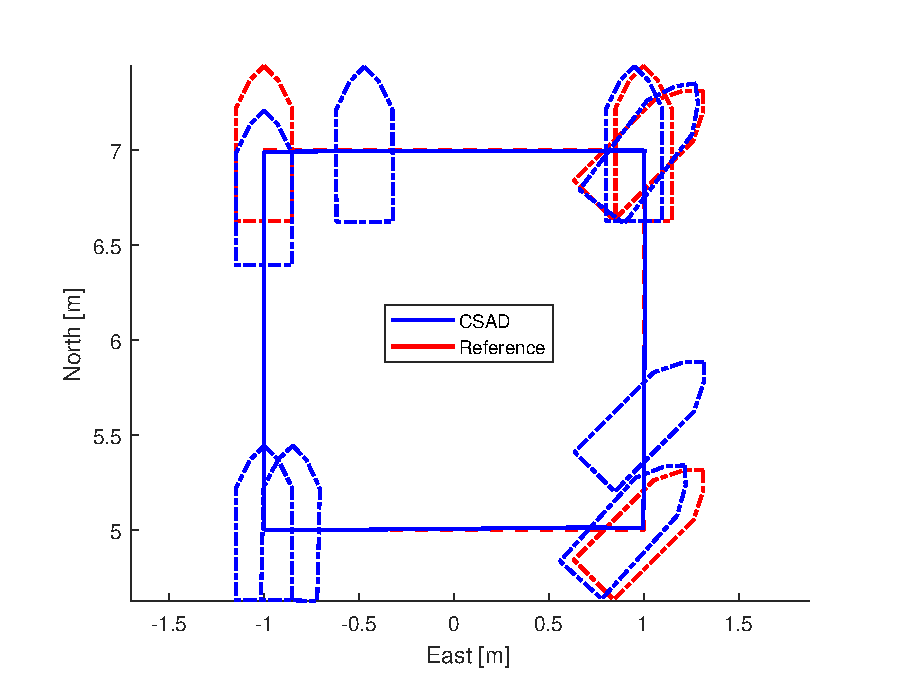
\includegraphics[width=1\textwidth]{plots/L1pose_sim.eps}
\caption{L1 simulated 4corner test}
\label{fig:sime4c}
\end{figure}

\begin{figure}[!h]
\centering
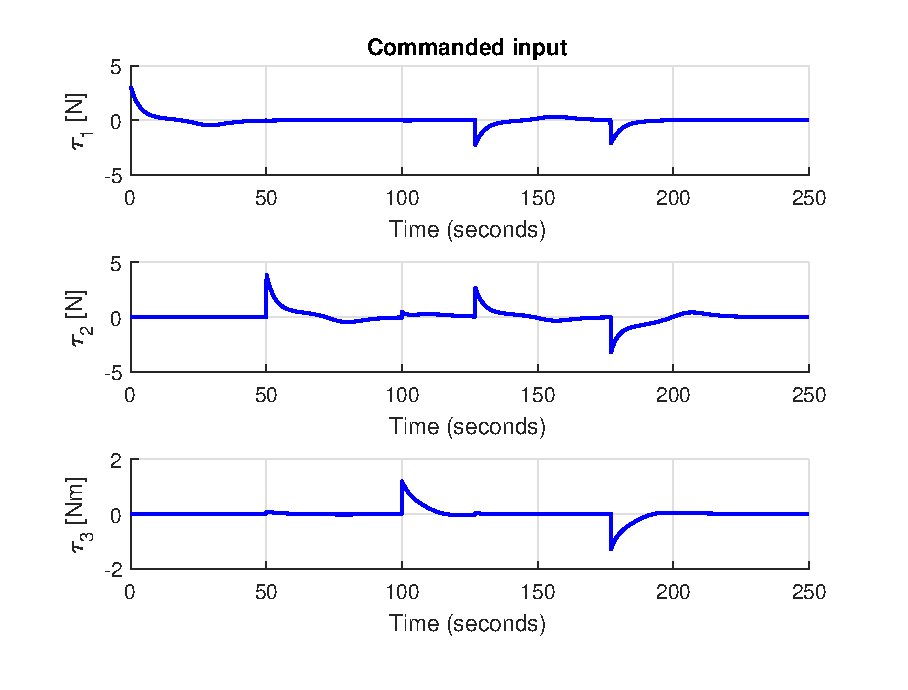
\includegraphics[width=1\textwidth]{plots/L1tau_sim.eps}
\caption{L1  - simulated control input}
\label{fig:simtau}
\end{figure}

\begin{figure}[!h]
\centering
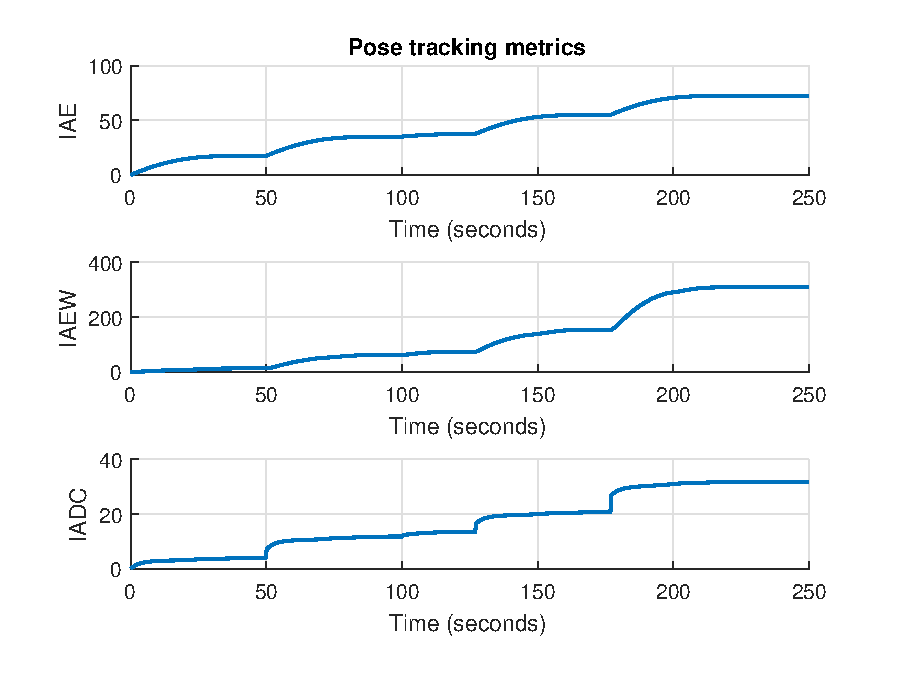
\includegraphics[width=1\textwidth]{plots/L1metrics_sim.eps}
\caption{L1 - simulated pose metrics}
\label{fig:simmetric}
\end{figure}

\subsection{Summary}

\section{Discussion}